\usetikzlibrary{decorations.pathmorphing}
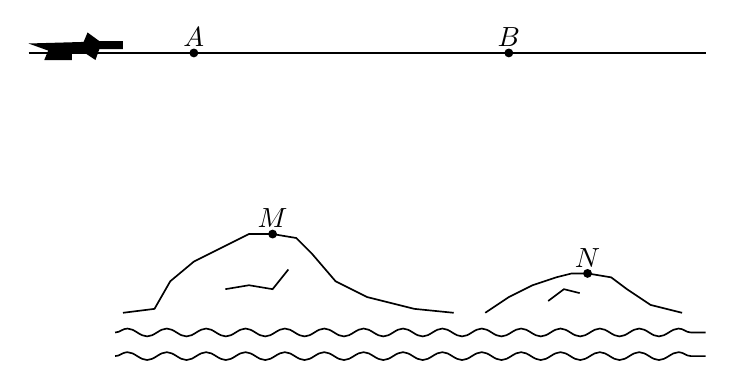
\begin{tikzpicture}[x=1cm,y=1cm,font=\normalsize,line width=.6pt]
% flight line
\coordinate (FL) at (-0.6,3);
\coordinate (FR) at (8,3);
\coordinate (A) at (1.5,3);
\coordinate (B) at (5.5,3);
\coordinate (M) at (2.5,0.7);
\coordinate (N) at (6.5,0.2);
\draw (FL) -- (FR);
% plane glyph (filled silhouette, schematic) at left end pointing left
\fill (FL) ++(0,0.12) -- ++(0.7,0.02) -- ++(0.05,0.12) -- ++(0.15,-0.11) -- ++(0.3,0) -- ++(0,-0.1) -- ++(-0.3,0) -- ++(-0.05,-0.14) -- ++(-0.15,0.1) -- ++(-0.15,-0.02) -- ++(0,-0.08) -- ++(-0.35,0) -- ++(0.05,0.12) -- cycle;
% dots A,B
\fill (A) circle (1.6pt);
\fill (B) circle (1.6pt);
\node[above=2pt,inner sep=0pt] at (A) {$A$};
\node[above=2pt,inner sep=0pt] at (B) {$B$};
% mountain M silhouette (jagged)
\draw (0.6,-0.3) -- (1.0,-0.25) -- (1.2,0.1) -- (1.5,0.35) -- (1.9,0.55) -- (2.2,0.7) -- (2.5,0.7) -- (2.8,0.65) -- (3.0,0.45) -- (3.3,0.1) -- (3.7,-0.1) -- (4.3,-0.25) -- (4.8,-0.3);
\draw (1.9,0.0) -- (2.2,0.05) -- (2.5,0.0) -- (2.7,0.25);
% mountain N silhouette
\draw (5.2,-0.3) -- (5.5,-0.1) -- (5.8,0.05) -- (6.1,0.15) -- (6.3,0.2) -- (6.5,0.2) -- (6.8,0.15) -- (7.0,0.0) -- (7.3,-0.2) -- (7.7,-0.3);
\draw (6.0,-0.15) -- (6.2,0.0) -- (6.4,-0.05);
% ground wavy base
\draw[decorate,decoration={snake,amplitude=0.5mm,segment length=5mm}] (0.5,-0.55) -- (8,-0.55);
\draw[decorate,decoration={snake,amplitude=0.5mm,segment length=5mm}] (0.5,-0.85) -- (8,-0.85);
% peak dots and labels
\fill (M) circle (1.6pt);
\fill (N) circle (1.6pt);
\node[above=2pt,inner sep=0pt] at (M) {$M$};
\node[above=2pt,inner sep=0pt] at (N) {$N$};
\end{tikzpicture}
